\chapter{Introduction}
\label{sec:org9288afb}
Dans cet ebook (ou livre électronique en bon français), vous allez
découvrir ce qui est bien trop souvent passé sous silence dans les
cours de langues\ldots{}, la phonétique ! En effet, en France en
particulier\footnote{N'ayant jamais fait d'études à l'étranger je ne
  peux pas me permettre de parler des autres pays}, les cours de
langues insistent rarement sur l'oral. Attention, je parle des cours
de langue avant le bac. Il faut savoir que \exFR{normalement}
l'objectif de l'enseignement obligatoire\footnote{En France
  l'instruction est obligatoire jusqu'à 16 ans ce qui correspond
  normalement à la classe de seconde ou première en cas de
  redoublement.} est d'atteindre le
\href{http://www.cambridgeenglish.org/fr/exams-and-tests/cambridge-english-certificate-cec/}{niveau
  B1} du cadre de référence européen. Hélas, la réalité est
loin d'être celle qu'espèrent les ministres et de nombreux indicateurs le prouvent :
\begin{itemize}
\item niveau en anglais par rapport aux autres pays
  \href{https://www.ef.fr/epi/regions/europe/}{européens}\footnote{Vous
    pouvez aller directement sur le site
    \url{https://www.ef.fr/epi/regions/europe/} pour observer l'étude complète.}(derrière l'Espagne, la Grèce, la Bulgarie, la Roumanie\ldots{} voir la figure
  \ref{fig:1} page \pageref{fig:1} pour plus de détails)
  \begin{figure}[h]
    \centering
    \caption[L'anglais en Europe]{Niveau d'anglais des
      pays européens}\vspace{.1cm}
    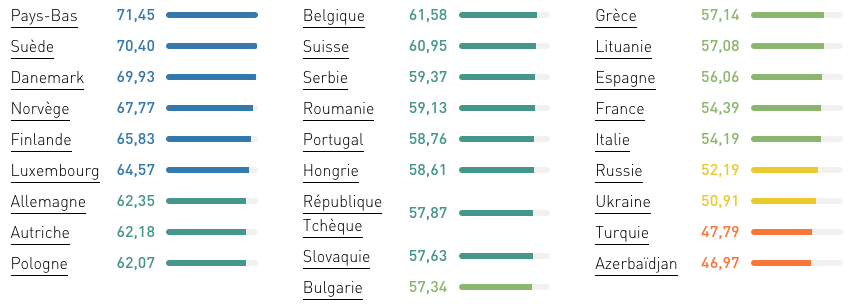
\includegraphics[scale=.5]{french-english-level-in-europe}
    
    \label{fig:1}
  \end{figure}
\item niveau en anglais par rapport \href{https://www.ef.fr/epi/}{au
    reste du monde}\footnote{Vous pouvez aller directement sur le site
  \url{https://www.ef.fr/epi/} pour observer l'étude complète}
(derrière la République Dominicaine et la Corée du Sud s'il vous
plaît\ldots{} voir la figure \ref{fig:2} page \pageref{fig:2} pour
plus de détails)
  \begin{figure}[h]
    \centering
    \caption[L'anglais dans le monde]{Niveau d'anglais dans le monde}\vspace{.1cm}
    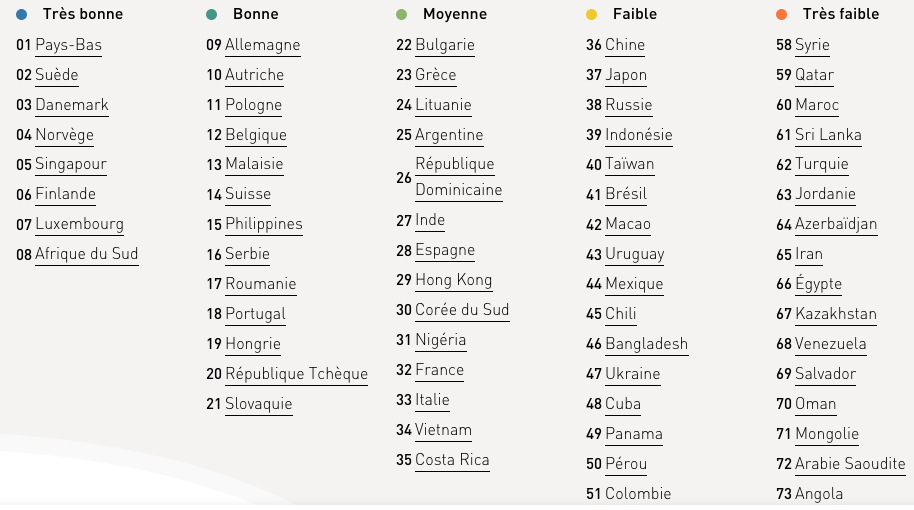
\includegraphics[scale=.5]{english-level-in-the-world}
    
    \label{fig:2}
  \end{figure}
\item encore des
  \href{https://www.digischool.fr/international/tests-anglais/chiffres-cles-francais-langues-etrangeres-16265.html}{chiffres
    accablants}\footnote{Vous pouvez lire l'article complet sur le
    site
    \url{https://www.digischool.fr/international/tests-anglais/chiffres-cles-francais-langues-etrangeres-16265.html}}
    (1/5 des français parlent anglais couramment voir la figure
    \ref{fig:3} page \pageref{fig:3} pour plus de détails.)
  \begin{figure}[h]
    \centering
    \caption[L'anglais en France]{Niveau d'anglais en France}\vspace{.1cm}
    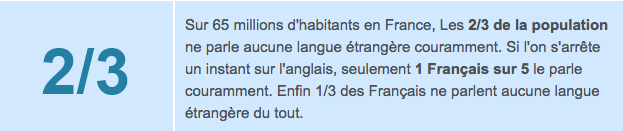
\includegraphics[scale=.725]{french-english-level-in-france}
    
    \label{fig:3}
  \end{figure}
\end{itemize}
Loin de moi l'idée de vous assommer avec des chiffres et encore moins
de partir dans l'auto-flagellation. Néanmoins, il faut être lucide, il
y a un problème franco-français (qui est très bien expliqué dans cet
\href{http://www.larevuedesressources.org/les-francais-et-les-langues-etrangeres,2920.html}{essai}). 
Ce problème est très bien développé et analysé dans l'essai du
professeur Daniel Emilio Rojas\footnote{Lisez-le c'est gratuit, très
  bien écrit et instructif : \url{http://www.larevuedesressources.org/les-francais-et-les-langues-etrangeres,2920.html}} (hispanophone natif qui parle et écrit
probablement beaucoup mieux le français que 90\% d'entre
nous). Cependant, je me permettrais de vous proposer un raccourci
(forcément réducteur) pédagogique en vous rappelant un fait
élémentaire mais que l'on oubli trop souvent. Parfois les solutions
sont tellement \exFR{bêtes} qu'on oubli d'y penser. Attention, je ne
prétends pas vous proposer de recette miracle. L'anglais est une
langue difficile\footnote{Claude Hagège, linguiste et professeur
  au Collège de France, l'explique dans cette vidéo
  \url{https://youtu.be/fjAuHvOMXFE} }, bizarre, complexe et illogique
(comme beaucoup de langues et notamment le français); et je ne suis
pas le seul à le dire puisque certains anglophones natifs (et
linguistes de surcroît) le disent et l'écrivent dans cet \href{https://aeon.co/essays/why-is-english-so-weirdly-different-from-other-languages}{article} qui permet également d'être
écouté\footnote{Comme je le montre dans cette vidéo
  \url{https://youtu.be/6wLbtx2iL7c}}. Donc oui l'anglais est
difficile, \textcolor{red}{mais} avec un peu de bon sens et de persévérence
vous pouvez y arriver\footnote{Bon, il y a une triste vérité qu'il
  faut accepter, vous ne parlerez \textcolor{red}{jamais} comme un natif (\textcolor{green}{sauf}
  si vous décidez de vous installer dans un pays anglophone).}. 

Mais quel est donc ce truc \exFR{tout bête} que l'on oublierait et dont je
ne vous ai toujours pas parlé ? Minute papillon ! Non ! Je n'essaie
pas de noyer le poisson, je vais vous révéler mon \exFR{truc}. Je vous
préviens, vous allez être probablement déçu, mais pourtant c'est une
évidence. \par
Allons-y ! Et bien, je ne sais pas pour vous mais pour moi (et il me
semble pour la plupart des gens aussi), l'acquisition de ma langue
maternelle a commencé par l'oral et non par l'écrit. Pendant au moins
5 ans (avant de rentrer au CP ou tout autre système scolaire qui
apprend à lire et à écrire), j'ai pratiqué en priorité l'écoute et la
méthode essai/erreur (en anglais on dit \exEN{try and guess} ce qui veut
dire \exFR{essayer et deviner}, qui est un point de vue plus positif). Ben
oui, quand on est enfant on baigne dans un environnement linguistique
oral. Et dès les premiers mois de la vie on essaie (avec beaucoup de
difficultés au début) de produire ou plutôt reproduire des sons que
l'on a entendu. Et croyez-moi, si vous avez oublié allez faire un tour
chez votre frère, soeur, cousin, cousine, ami, amie qui a (ont) des
enfants en bas âge et cela vous raffraichira la mémoire. La parole est
si importante pour l'humanité qu'elle a été pendant des siècles ( des
millénaires même!) le seul et unique vecteur de
communication. D'ailleurs aujourd'hui encore parmi les presque 7~000
\href{http://www.museedelhomme.fr/fr/combien-langues-sont-parlees-monde}{langues dans le monde} la plupart ne possèdent pas de système
d'écriture. Pour plus de précisions sur la répartition linguistique
dans le monde vous pouvez consulter \href{http://www.axl.cefan.ulaval.ca/Langues/1div\_recens.htm}{ce site canadien} qui tire ses
sources statistiques du \textcolor{red}{Summer Institute of Linguistics} du
Texas\footnote{Voici l'url du site
  \url{http://www.axl.cefan.ulaval.ca/Langues/1div_recens.htm}}
(2017).\par


\begin{quote}
Les Romains, déjà, ne parlaient pas exactement la langue qu'ils
écrivaient. Ainsi, \exFR{cheval} vient d'un mot parlé, \exFR{caballus}, alors
que le latin classique écrit \exFR{equus} -- d'où viendront des mots <<~savants~>> comme \exFR{équidé} et \exFR{équitation}
\end{quote}\footnote{Extrait du livre \href{https://www.amazon.fr/gp/product/2844100015/ref=as\_li\_tl?ie=UTF8\&camp=1642\&creative=6746\&creativeASIN=2844100015\&linkCode=as2\&tag=wwwbecomefree-21\&linkId=985f3a849fd44728e8480993cf2d5490}{français lycée} de Pierre Brunel.}

D'ailleurs comme le montre \href{https://youtu.be/Wn\_eBrIDUuc}{cette vidéo}, les zones du cerveau actives
pour la parole et pour l'écriture sont différentes.\par

\begin{quote}
Longtemps, le français s'est écrit comme il se parlait; vice versa,
toutes les lettres se prononçaient, comme en latin. La notion même
d'orthographe n'existait pas.
\end{quote}\footnote{Extrait du livre
\href{https://www.amazon.fr/gp/product/2844100015/ref=as\_li\_tl?ie=UTF8\&camp=1642\&creative=6746\&creativeASIN=2844100015\&linkCode=as2\&tag=wwwbecomefree-21\&linkId=985f3a849fd44728e8480993cf2d5490}{français
  lycée} de Pierre Brunel.}


En lisant cet extrait je pari que certains d'entre vous sont en train
de chercher un moyen pour inventer une machine à remonter le temps. 

Vous vous demandez sûrement où je veux en venir. Mon but est de vous
faire comprendre ou plutôt de vous rappeler qu'une langue ça s'écoute
et ça se parle pendant un certain temps (jusqu'à ce que ça devienne
naturel) avant d'apprendre à l'écrire et d'étudier toutes les
subtilités de la grammaire. \href{https://fr.wikipedia.org/wiki/Django\_Reinhardt}{Django Reinhardt} et \href{https://fr.wikipedia.org/wiki/Louis\_Armstrong}{Louis Amstrong} ne
savaient ni lire ni écrire la musique et pourtant ils sont des
musiciens vénérés de leur vivant et encore aujourd'hui.\par

Et oui une langue c'est également une musique ! Une langue a une
musicalité et un rythme. Pas de chance pour nous le français (ou
plutôt le \exFR{parisien}\footnote{Lire la section~\ref{sec:lat2fr}
  page~\pageref{sec:lat2fr} pour plus d'explications.})
n'est pas très chantant. Mais pourtant si l'on écoute les accents du
midi il y a tout de suite plus de mélodies qui chatouillent nos
oreilles. 

En résumé, ce que je vais partager avec vous dans ce livre, ce
sont les sons de la langue anglaise. Les 45 sons (certains en
décrivent 44, pour le français\footnote{Selon le
  \href{https://www.amazon.fr/gp/product/221010632X/ref=as_li_tl?ie=UTF8&camp=1642&creative=6746&creativeASIN=221010632X&linkCode=as2&tag=wwwbecomefree-21&linkId=c8c522ee07ffc9188dd9a768e39d88e0}{Grévisse
  de l'enseignant} il y a 36 sons <<~\exFR{purement}~>> français
auquel on ajoute le son [ŋ] hérité de l'anglais et notamment utilisé dans \exEN{parking}.} c'est pareil, certains disent 36
d'autres 37).\par
\begin{itemize}
\item Dans une première partie je vous présenterai la phonétique du
français. En effet, il me semble plus judicieux d'approcher ce nouvel
ensemble de symbole qui décrit les sons avec précisément des sons que
vous utilisez déjà tous les jours.  Pour conclure cette partie je
rappelerai deux faits qu'il faut \textcolor{red}{absolument garder à l'esprit} :
\begin{enumerate}
\item Le français est une langue syllabique alors que l'anglais est
  une langue accentuelle\footnote{Ce canadien francophone l'explique
    très bien dans cette
    \href{https://youtu.be/EjVHGsRCf8M?t=4m45s}{vidéo}.}.
\item En français il y a 36 sons\footnote{Selon le
  \href{https://www.amazon.fr/gp/product/221010632X/ref=as_li_tl?ie=UTF8&camp=1642&creative=6746&creativeASIN=221010632X&linkCode=as2&tag=wwwbecomefree-21&linkId=c8c522ee07ffc9188dd9a768e39d88e0}{Grévisse
  de l'enseignant} selon Sousa il n'y en aurait que 32. Pour ce
chiffre j'accorderai plus de crédit au Grévisse pour la bonne et
simple raison qu'en tant que linguiste francophone il me semble plus
compétant que Sousa qui est anglophone.} et 250 façons\footnote{Encore une
fois les estimations diffèrent
\href{https://www.amazon.fr/gp/product/221010632X/ref=as_li_tl?ie=UTF8&camp=1642&creative=6746&creativeASIN=221010632X&linkCode=as2&tag=wwwbecomefree-21&linkId=c8c522ee07ffc9188dd9a768e39d88e0}{Grévisse}
n'en compte que 130 ce qui accentue encore plus la complexité de l'anglais.} de les écrire alors
  qu'en anglais il y a 44 sons pour 1~100 façons de les
  écrire\footnote{Les chiffres concernant les façons d'écrire sont
    issus des comparaisons présentées dans le livre
    \href{https://www.amazon.fr/gp/product/B00M0GDXN8/ref=as_li_tl?ie=UTF8&camp=1642&creative=6746&creativeASIN=B00M0GDXN8&linkCode=as2&tag=wwwbecomefree-21&linkId=e782cf430858413ec9135fcef1644b20}{How
      The Ell Brain Learns} Chapter 4 Teaching English Language
    Reading and Writing page 84 Table 4.1.}.
\end{enumerate}
Par conséquent \underline{la prononciation, l'accent et le rythme} ne sont pas
superflus mais \textcolor{red}{\underline{obligatoire en anglais}}.\par

\item Dans une deuxième partie je vais vous présenter 45 sons qui sont absolument
\textcolor{red}{fondamentaux} dans la langue anglaise. En insistant
particulièrement sur ceux qui n'apparaissent pas du tout dans la
langue française. Et pour bien faire la différence il était important
de commencer par la phonétique de la langue française que vous ne
connaissez probablement pas encore. C'est pour cette raison qu'il est
vivement recommandé de lire ce livre dans l'ordre.
\end{itemize}
J'ai dit qu'on apprend d'abord à parler avant d'écrire, c'est vrai,
mais a priori, si vous lisez ce livre c'est que vous savez lire. Et
comme vous savez lire et bien on va en profiter pour apprendre encore
plus efficacement en utilisant
l'\href{https://fr.wikipedia.org/wiki/Alphabet\_phon\%25C3\%25A9tique\_international}{API}\footnote{Vous
pouvez le consulter sur Wikipédia \url{https://fr.wikipedia.org/wiki/Alphabet_phon\%C3\%A9tique_international}}
(Alphabet Phonétique International). En anglais on l'écrit
IPA\footnote{Vous pouvez également consulter la version anglaise de
  Wikipédia \url{https://en.wikipedia.org/wiki/International_Phonetic_Alphabet}}
(International Phonetic Alphabet).\par

Et cerise sur le gâteau, ceci
vous sera utile pour toutes les autres langues que vous souhaitez
apprendre ou que vous parlez déjà (cela va même améliorer votre
français\footnote{Vous pouvez déjà vous entraîner grauitement grâce
  aux cartes mémoires que j'ai créé : \url{https://tiny.cards/decks/6YTEvyrN/english-phonetics}} !). D'ailleurs, contrairement à ce que certaines personnes
pourraient penser, apprendre une autre langue, et en particulier
l'anglais, améliore votre niveau de français\footnote{En effet il existe plus de 25~000 mots anglais
  d'origine française et vous pouvez en découvrir quelques-uns grâce
  aux cartes mémoires que j'ai créé :
  \url{https://tinycards.duolingo.com/decks/6VNKUdba/english-words-with-french-origin}
et au livre plus complet \href{https://www.amazon.fr/gp/product/225315444X/ref=as_li_tl?ie=UTF8&camp=1642&creative=6746&creativeASIN=225315444X&linkCode=as2&tag=wwwbecomefree-21&linkId=5317e7b0e063b4d6c7c676b11420e49d}{Honni soit qui mal y pense} }. Ce n'est pas magique,
mais c'est véridique. Alors c'est parti, allons découvrir les 45 sons
de la langue anglaise (qui n'a plus grand chose à voir avec
Shakespeare de la même manière qu'on ne parle plus la langue de
Molière).